% arara: pdflatex
\documentclass{report}
\usepackage{graphicx}
\usepackage{xcolor}
\usepackage{forest}
\usepackage{amsmath}
\renewcommand{\chaptername}{Section}
\begin{document}
\begin{titlepage}
\begin{center}
	\vspace*{1cm}

	\Huge
	\textbf{Course Project}

	\vspace{0.5cm}
	\LARGE
	Second Deliverable: The Parser	

	\vspace{1.5cm}

	\textbf{Quin'darius Lyles-Woods}
	\Large
	qlyleswo@students.kennesaw.edu

	\vfill
	\LARGE
	Concepts of Programming Languages	\\
	Professor Jose Garrido			\\
	Section W01 				\\
	4308
	\vspace{0.8cm}

	
\includegraphics[width=\textwidth]{kennesawlogo}

	\vspace{0.8cm}

	\Large
	Bachelors of Computer Science\\
	Kennesaw State University\\
	1100 South Marietta Pkwy SE\\
	Marietta, GA 30060\\
	\today	

	\vspace{1cm}

\end{center}
\end{titlepage}


\section*{Task}
The development of an Ada program for exploring the properties of complex numbers. 

\vspace{0.5cm}

\subsection*{Assignment Goals}
\begin{itemize}

	\item Author a complex numbers package in Ada.
	\item Write a report on the development of such a package.
	\item Have the following operations; addition, subtraction, multiplication, and division. 
\end{itemize}

\subsection*{Source Code}
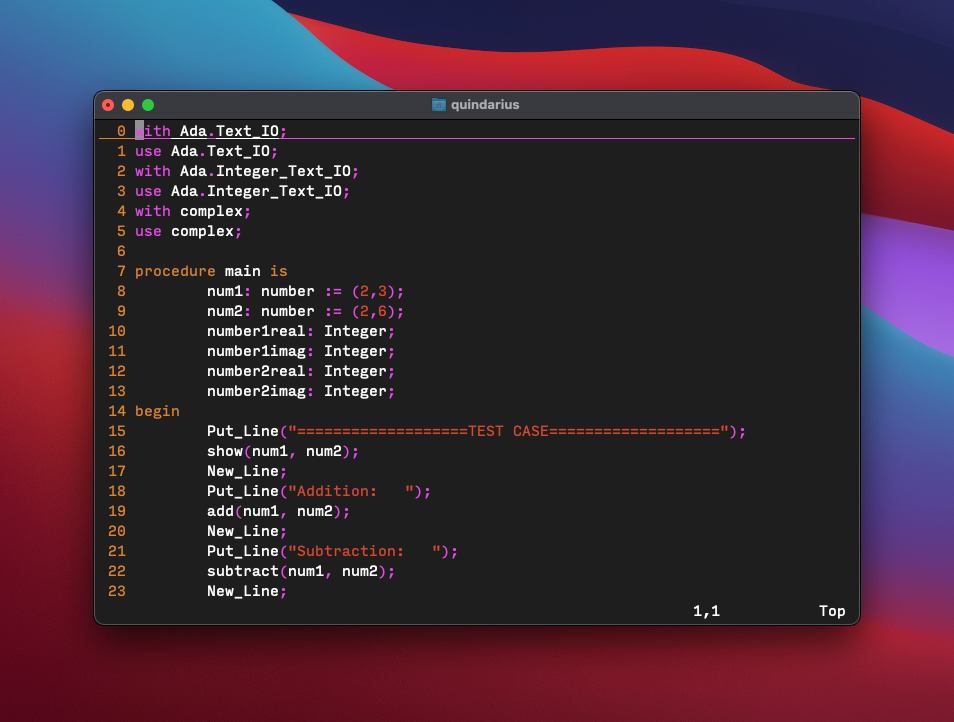
\includegraphics[width = \textwidth]{images/ada1}
\subsection*{Compile Output}
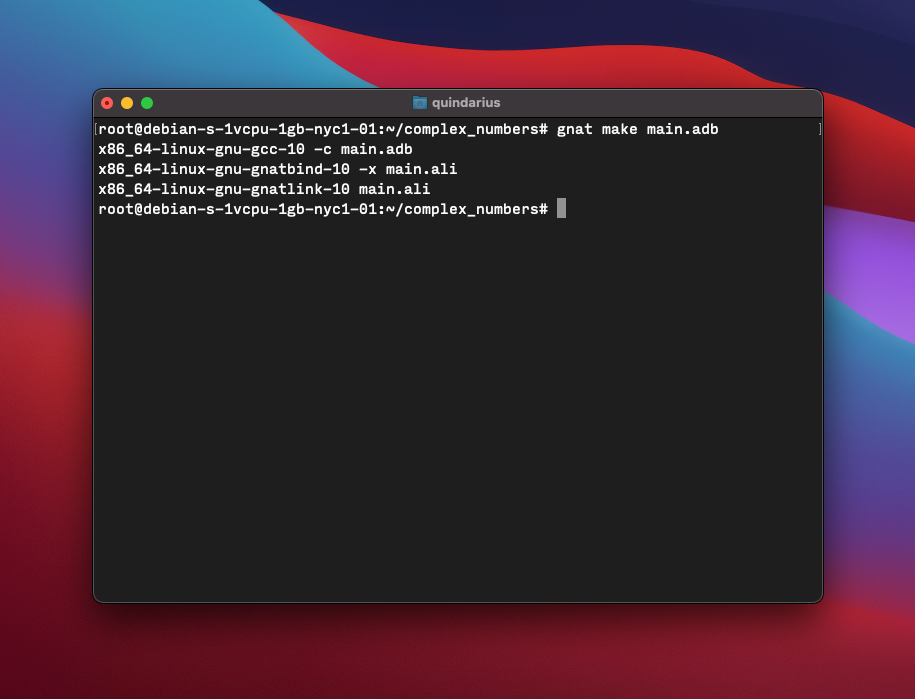
\includegraphics[width = \textwidth]{images/ada2}
\subsection*{Test Output}
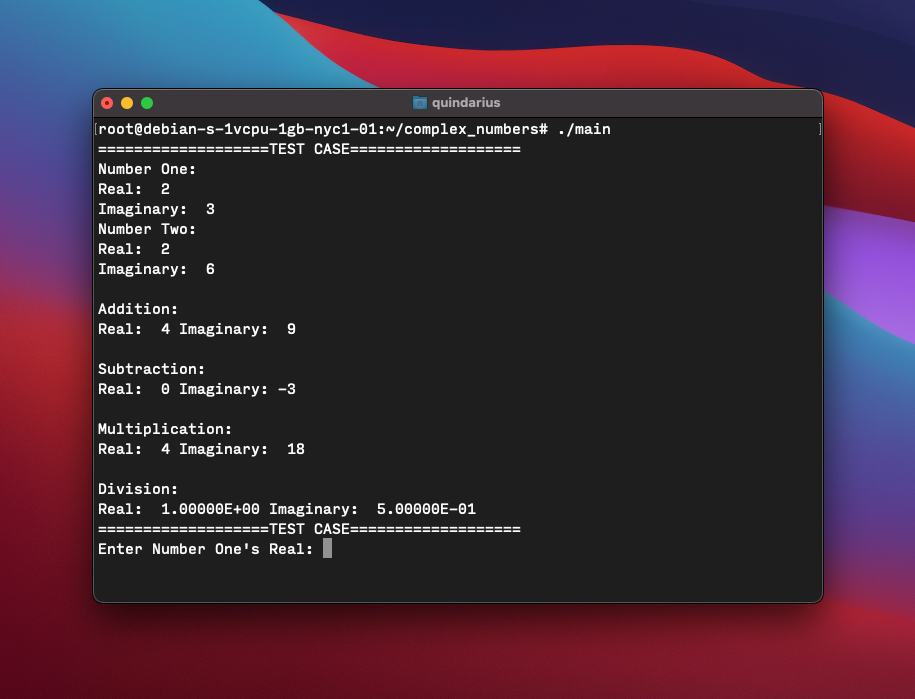
\includegraphics[width = \textwidth]{images/ada3}
\subsection*{User Input Output}
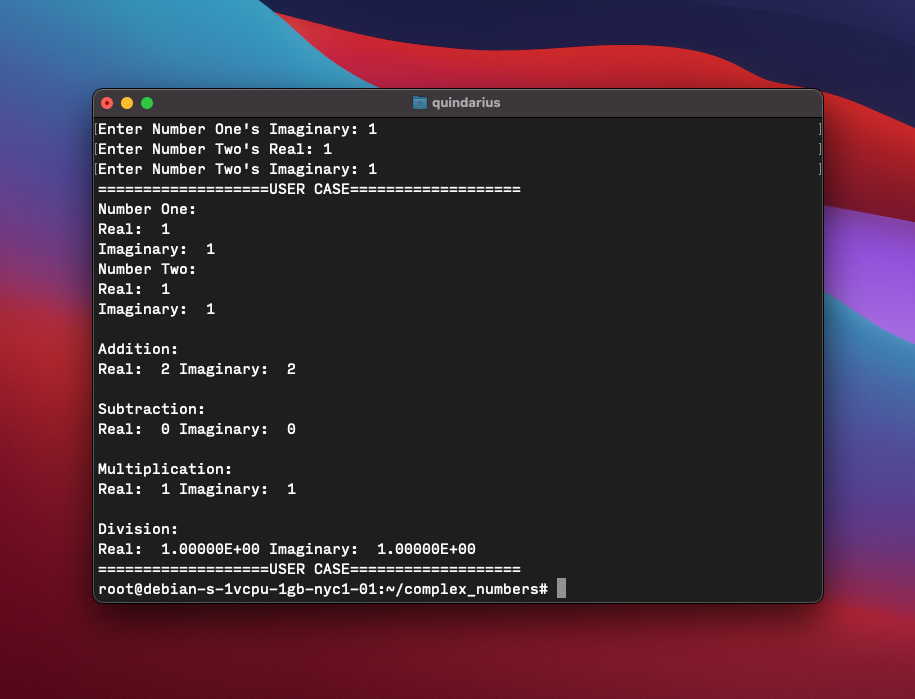
\includegraphics[width = \textwidth]{images/ada4}

\section{Summary}
After finishing this assignment I have a better understanding on how Ada works. Defiantly not my favorite experience but I loved how it resembled c with adding external code. 
Another notation about the language that I might what to follow in my other programs is the stark distinction of where declaration and operational code was within. 
They don't even allow the two to mix and I think that is a plug in the long run for the language design. 
Luckily for me, that more of a style aspect in other language and I will be able to take that style and put it almost anywhere. 

Lastly, this assignment allowed me to review complex numbers.
They are so simply but for some reason have been seen as almost mystical to me. 
So I appreciated that aspect of the assignment as well.
\end{document}

